\chapter{Implementation and Performance of GAIA}
\newthought{The standard algorithms} for $b$ and $c$-jet tagging in the High Energy Physics community are MV1 and JetFitterCombNN respectively -- two neural networks batch trained using a variety of \emph{upstream} information about the particle collisions. Using the same features -- some basic likelihoods, vertexing information, and other signatures -- we show a significant improvement over MV1 and JetFitterCombNN. In addition, we show (albeit qualitatively) that the pretrained features extracted via the Stacked Denoising Autoencoder cluster and show separation between bottom and light jets. First, we provide a brief description of the implementation of GAIA, then we discuss benchmarking and performance measures on the classification task.

\section{Design and Implementation of GAIA}
GAIA was implemented with speed, portability, modularity, and expandability in mind. In addition to development on the algorithms side -- i.e., Deep Learning, we integrate GAIA into the ROOT \citep{ROOT} Framework for High Energy Physics Data Analysis. Simulations and data within CERN are stored in a ROOT structure called a \texttt{TTree}. We provide a simple wrapper around the native CERN I/O system to make training, testing, and validation easier, and more in line with the mathematical formulation.

The GAIA framework was written in C++ using two standards for two separate parts. The main interface was written using C++11 standard. Specifically, the \texttt{<utility>} and \texttt{<memory>} headers were used for R-Value references and smart pointer (\texttt{std::unique\_{}ptr}) functionality, the \texttt{<random>} header was used for random number generation, and range-based for-loops were used, as the compiler used (GCC 4.8.X) optimized all iterations using this structure when the \texttt{-O3} flag is passed. The header-only thin-client library uses the C++0x standard to ensure compatibility with the existing CERN software.

We provide a \texttt{Layer} class which encapsulated all operations relating to equations \eqref{net_prediction} and \eqref{auto_soln}, allowing for functionality with or without feature learning. Specifically, the \texttt{Layer} class holds $W_i$ and $\mathbf{b}_i$ The \texttt{Layer} class also is responsible for all parameter manipulation, and offers methods for setting parameters such as learning rate, etc. For a presented input $\mathbf{x}$, the \texttt{Layer} class offers a method called \texttt{Layer.feed(std::vector<double> x)} which forms and stores $\mathbf{z^{(i)}} = W_i \mathbf{x}+\mathbf{a}_i$ and $\mathbf{a}^{(i)}=f(\mathbf{z^{(i)}})$. Also noteworthy is the fact that the activation function $f$ is passed as a function pointer to the method within the constructor, making user-preference for a specific type of activation function more feasible.

We also provide an \texttt{Architecture} class, which provides a generic method of combining arbitrarily sized \texttt{Layer} objects into a network structure. It also handles all data passing between layers, and mediates the greedy feature learning within the neural network. Its main purpose is to provide the backpropagation function to the neural network. Build on top of the \texttt{Architecture} class is a \texttt{NeuralNet} class, which provides API sugar around many of the methods and provided functionality. The \texttt{NeuralNet} class also provides a mediatory layer between the user and the \texttt{Dataset} class, which serves as the wrapper around the native CERN \texttt{TTree} data structure. Thus, a user will only need to interact with the \texttt{NeuralNet} class from data loading to training to testing. We now walk through a simple example to illustrate the functionality of the API. Suppose we have a ROOT file named \texttt{dataset.root} containing a \texttt{TTree} called \texttt{MyTree}. Suppose we want to predict the outcome called \texttt{"output"} from the variables called \texttt{"var\_1"}, \texttt{"var\_2"}, and \texttt{"var\_3"}, and all of these variables are within the \texttt{TTree} called \texttt{MyTree}. Now suppose we want to build a neural network with one hidden layer, say with two nodes. The following code will do this. 

\begin{small}
\begin{verbatim}
#include "NeuralNet.h"
#include <TFile.h>
#include <TTree.h>

int main(int argc, char const *argv[])
{
    // Make a neural net with 3 inputs, 2 hidden nodes
    // and one output
    std::vector<int> structure = {3, 2, 1};

    // Initialize the network
    NeuralNet Net(structure);

    // The first argument is the root file and
    // the second argument is the name of 
    // the TTree
    Net.set_dataset("dataset.root", "MyTree");

    // The first argument is the variable name
    // and the second argument is its numeric type
    Net.set_input_branch("var_1", "double");
    Net.set_input_branch("var_2", "double");
    Net.set_input_branch("var_3", "double");

    // Same for outputs.
    Net.set_output_branch("output", "double");

    // Find the transform so that inputs are of
    // zero mean and unit variance.
    Net.getTransform();

    // Train for 5 epochs, using 1000 points
    // and save the configuration to a file
    // called "neuralnetwork.nnet"
    Net.train(5, 1000, "neuralnetwork.nnet");

    return 0;
}

\end{verbatim}
\end{small}

As we can see, the interface is straight-forward, and additional functionality is elaborated upon in documentation. 

\section{Measuring Performance}


To benchmark the performance of GAIA with respect to the current selection of other particle classifiers,  we use some standard measures of classifier performance. We make these metrics very problem dependent for the sake of concreteness. We denote the quarks / jets that we try to identify as $\{b,c,u\}$ for Bottom, Charm, and Light jets respectively. These will be henceforth referred to as "flavors". For a given threshold -- called a "cut" within High Energy Physics -- on any number of output discriminants, define the efficiency of such a cut with respect to a certain flavor to be the number of jets of such a flavor that pass the discriminant out of the total number considered. We say that a jet or quark \emph{passes a cut} if its value of the discriminant is higher than the threshold or cut value.  Denote this efficiency quantity as $\epsilon_\theta$, for $\theta\in\{b,c,u\}$. This can be more succinctly formulated as
\begin{equation}
\epsilon_\theta = \frac{\text{\# of }\theta\text{ jets passing the cut in sample}}{\text{Total \# of }\theta\text{ jets in sample}}
\end{equation}
 with respect to some cut on some combination of discriminants. To measure purity, we also consider the \emph{rejection} of a cut with respect to some flavor $\theta$, $r_\theta$, which is simply defined as the reciprocal of the efficiency. That is $r_\theta = 1 / \epsilon_\theta$.
 
For a particular type of identification problem -- that is, for $c$-tagging or $b$-tagging, we always consider the efficiency of the signal and the rejection of the two backgrounds. For any level of signal efficiency, it is always desirable to maximize the background rejection for both types of background. 

For a physics analysis, we cannot simply take the Maximum A Posteriori (MAP) estimate of class membership, as different analysis groups need different levels of purity or yield, and some groups have a very different sample composition. For example, a group needing to identify $b$-jets against a background that is primarily $u$-jets is going to need a very different discriminant than an analysis group needing to separate $b$-jets from an even mix of $c$ and $u$-jets. 

Consider our particular classifier, with outputs $p_u, p_b$, and $p_c$ representing the posterior probabilities that an observation is a light jet, bottom jet, or charm jet respectively. The posterior space has a distribution $f_{p_u,p_b,p_c}(p_u, p_b, p_c)$ over all outputs, and individual distributions for each $\theta$, $f_\theta(p_\theta)$. Suppose our signal is $\theta$. We then can construct a set of discriminants
\begin{equation}
D = \{ \log(p_\theta / p_\nu) : \nu \in \{u,b,c\}, \nu \neq \theta \}.
\end{equation} 
In our particular case, this leaves two discriminants for a three class problem. Note that we take a $\log(\cdot)$ here simply to make any even sampled cuts on this distribution more evenly sampled. 

\subsection{Sensitivity to $p_T$ and $\eta$}

The usage of a classifier is relatively unique within physics. Since any classifier will have to probe and classify on datasets that are of different $p_T$ and $\eta$ ranges, care must be taken to ensure that a classifier isn't overfitting to a particular $(p_T,\eta)$ combination. Consider the following. Suppose we let a classifier learn the fact that low $p_T$ jets tend to be light jets and higher $p_T$ jets tend to be $b$-jets. 

\subsection{Choosing What to Learn}

Using \emph{online physics reweighting}, we can dictate what features our pretraining discovers. We can also dictate to what degree our \nn{} should balance out biases in distributions over the kinematic variables $p_T$ and $\eta$.

\section{$b$-tagging}

To measure performance

\begin{figure}
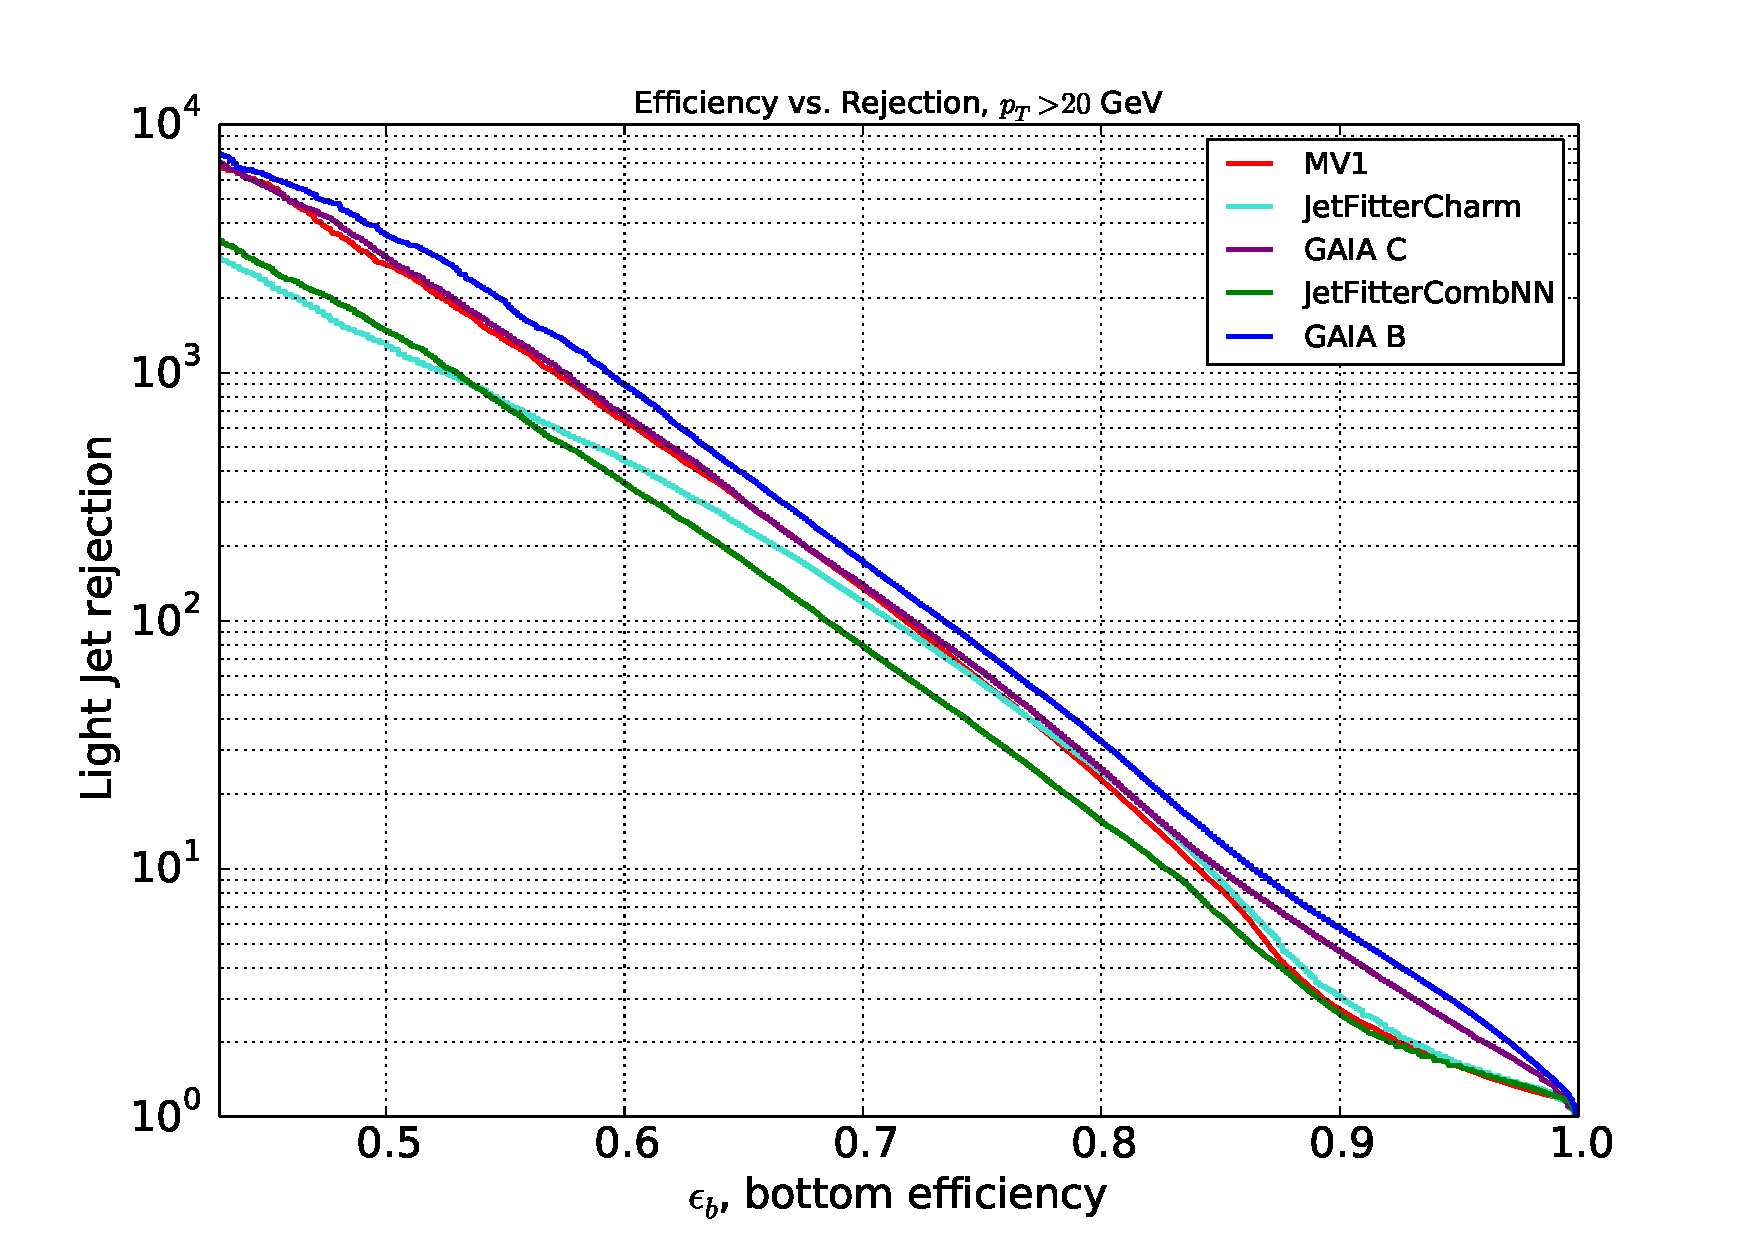
\includegraphics[width=\textwidth]{figures/btag/u_rej_ROC.pdf}
\caption[The ATLAS detector]{$u$-rejection Receiver Operating Characteristic Curve of Tagging Lineup.
\label{fig:urejROC}}
\end{figure}

\begin{figure}
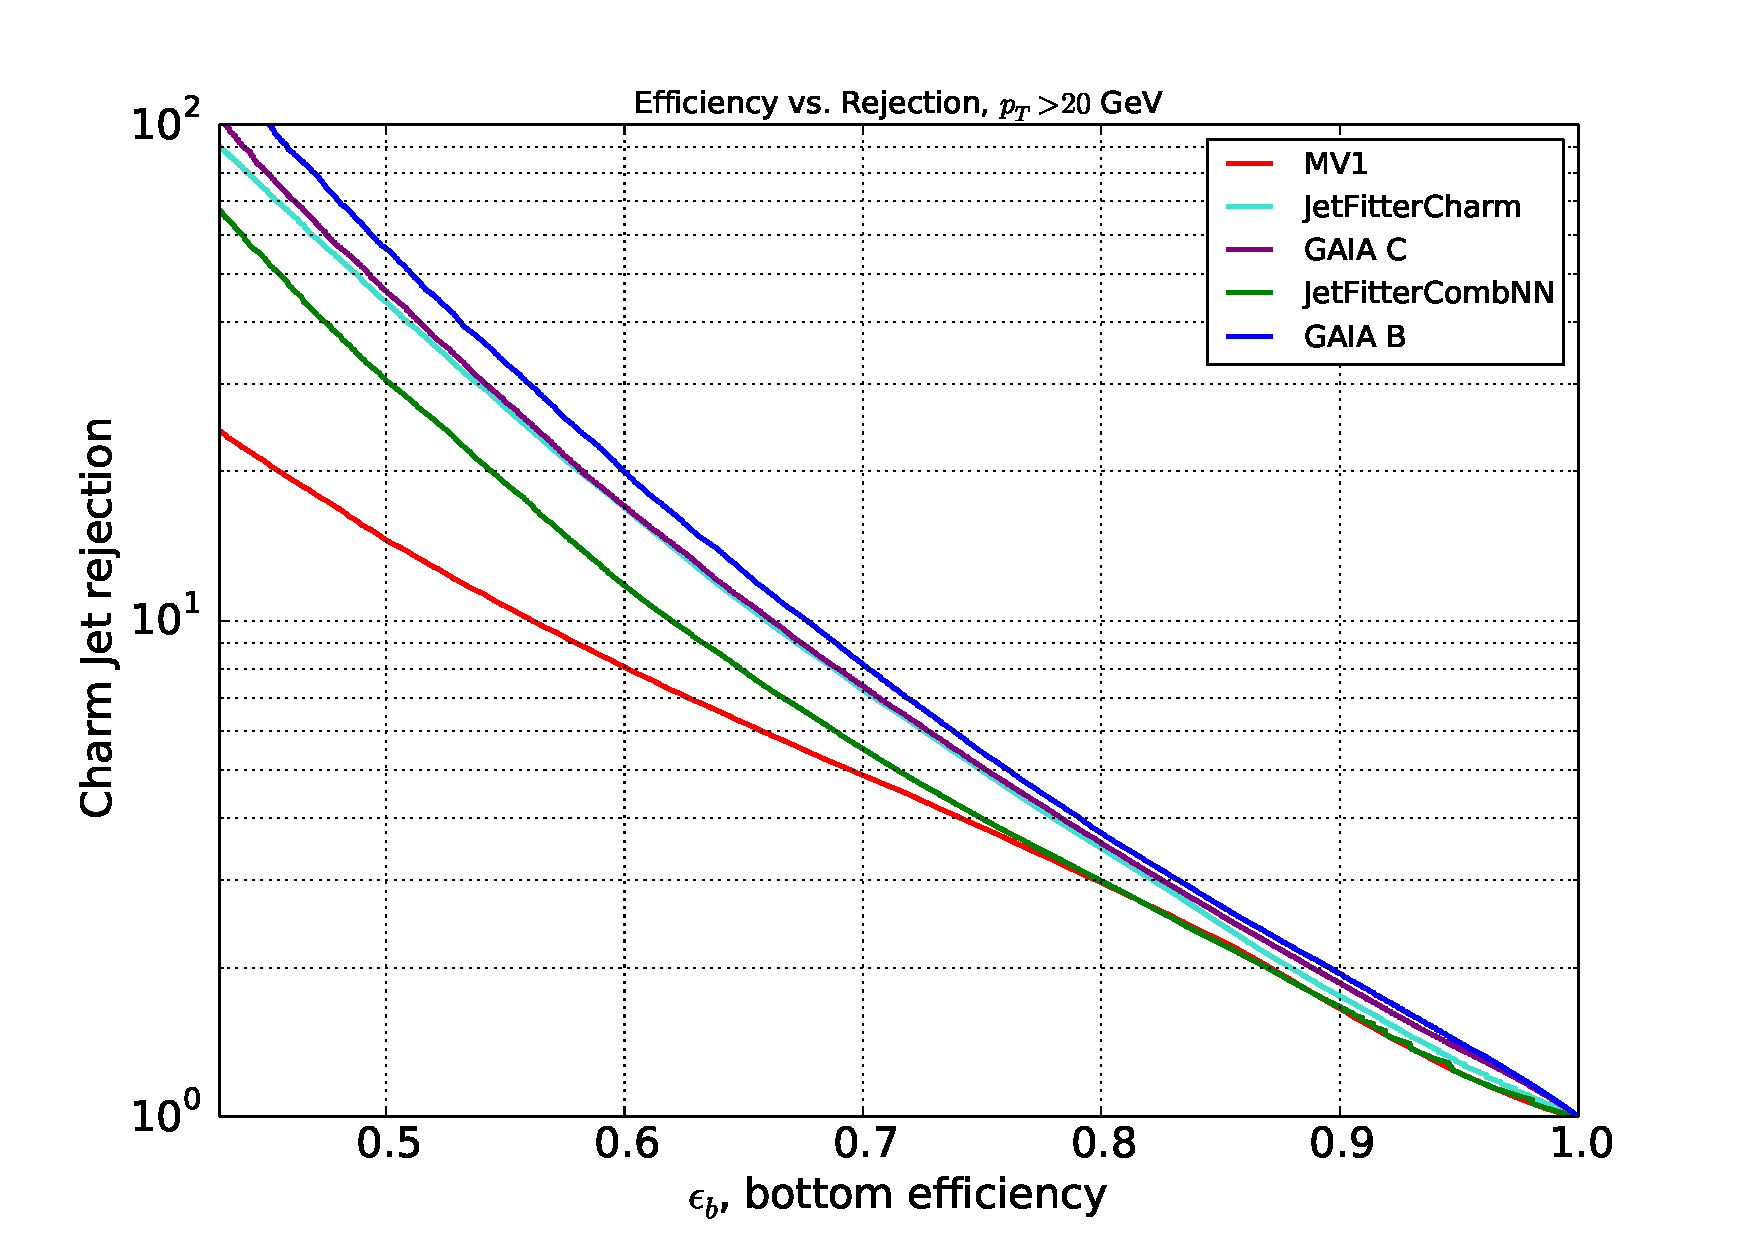
\includegraphics[width=\textwidth]{figures/btag/c_rej_ROC.pdf}
\caption[The ATLAS detector]{$c$-rejection Receiver Operating Characteristic Curve of Tagging Lineup.
\label{fig:crejROC}}
\end{figure}

\begin{figure}
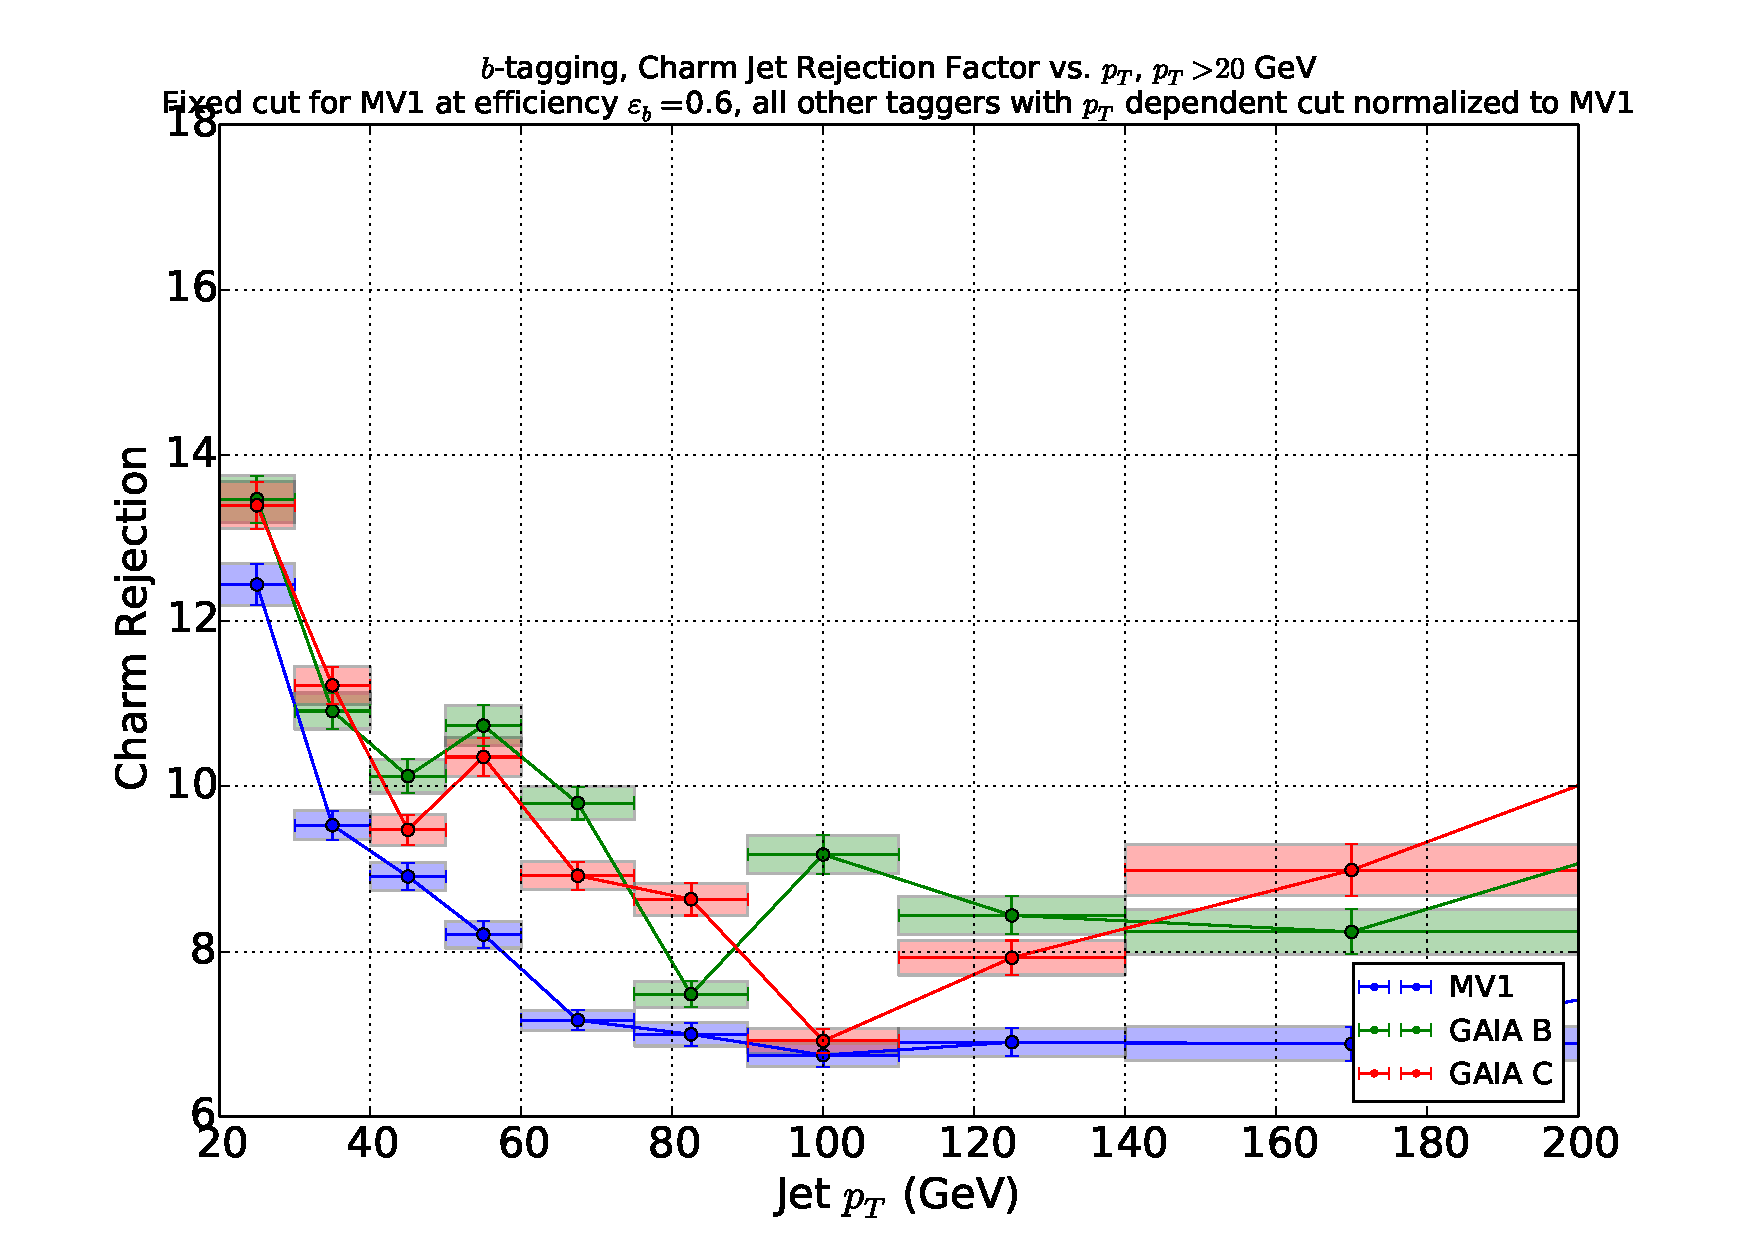
\includegraphics[width=\textwidth]{figures/btag/c_rej_mv1normalized_pTdep_60pct.pdf}
\caption[The ATLAS detector]{MV1 Normalized Performance of GAIA.
\label{fig:crejmv1norm60}}
\end{figure}

\begin{figure}
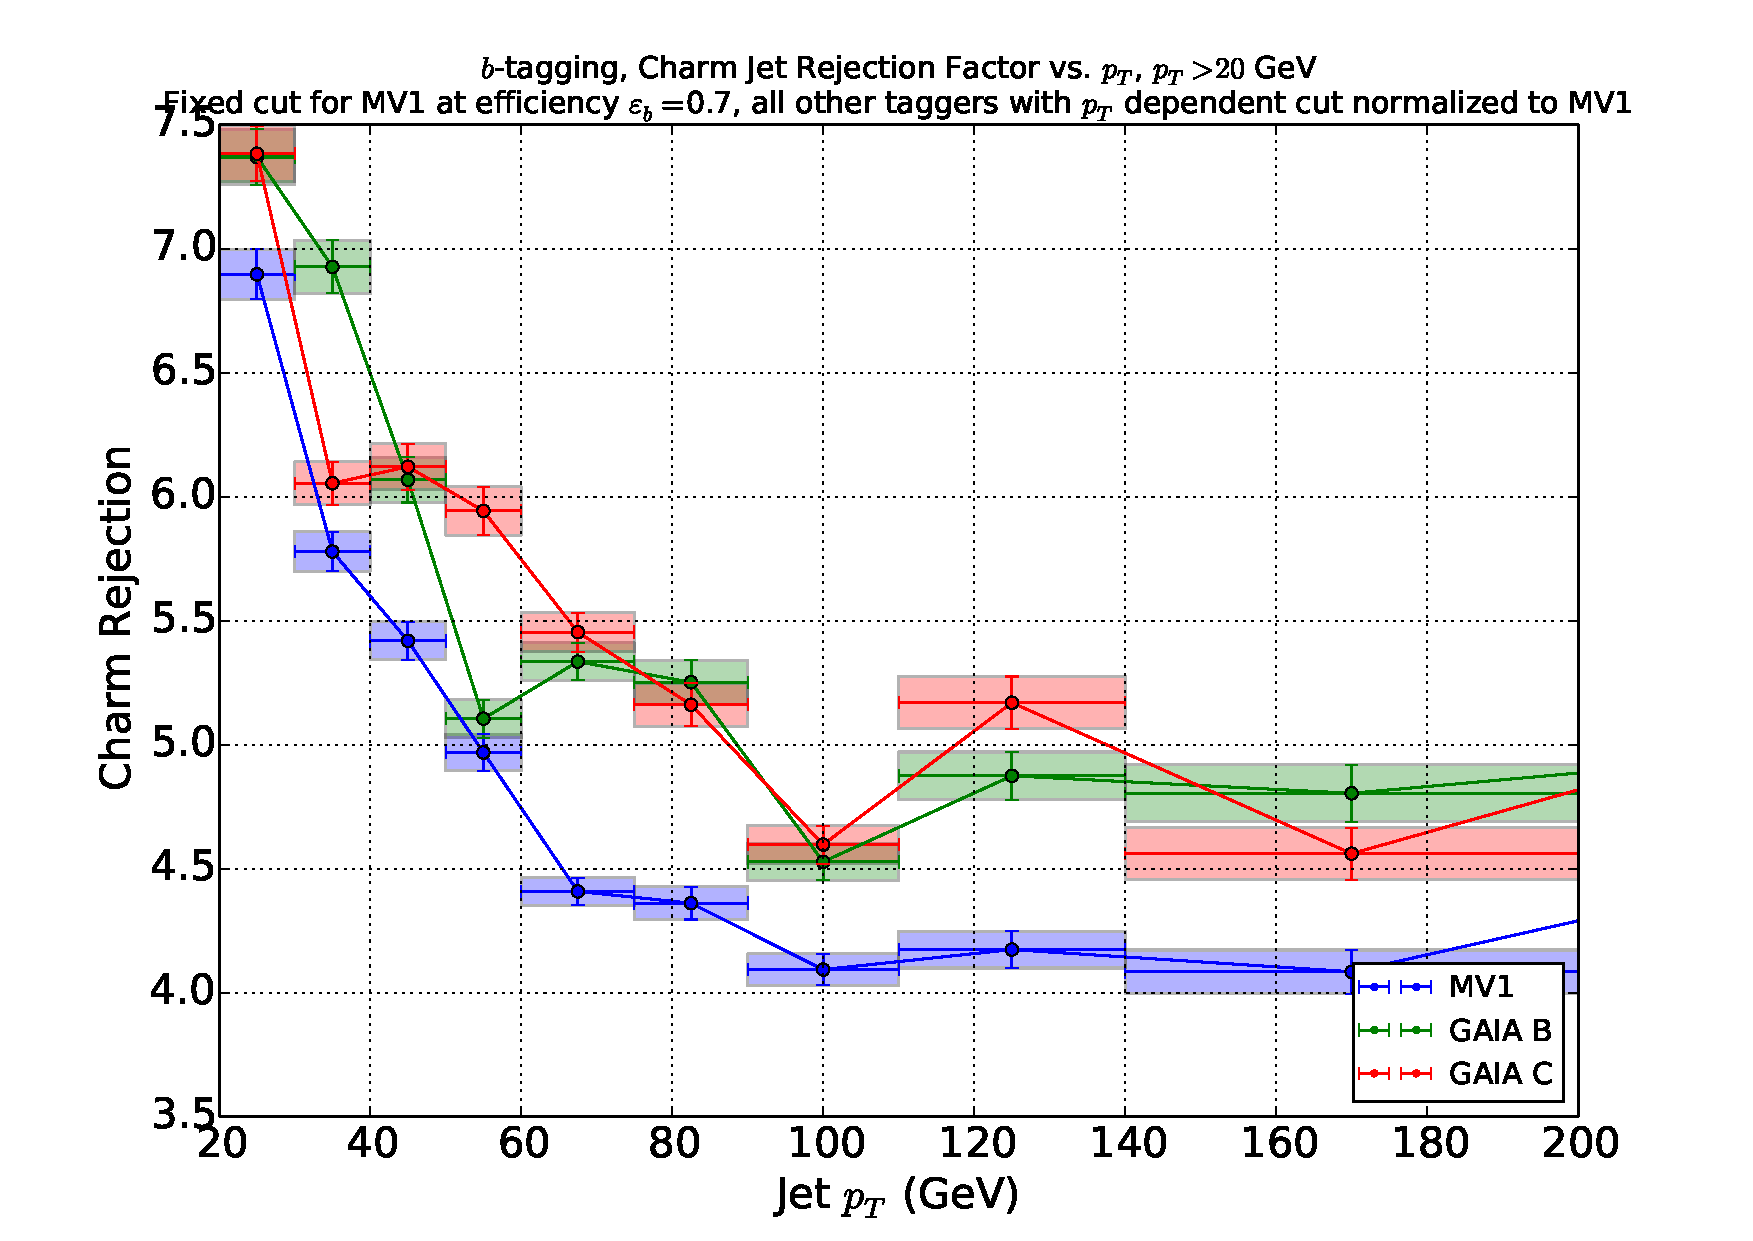
\includegraphics[width=\textwidth]{figures/btag/c_rej_mv1normalized_pTdep_70pct.pdf}
\caption[The ATLAS detector]{MV1 Normalized Performance of GAIA.
\label{fig:crejmv1norm60}}
\end{figure}


\begin{figure}
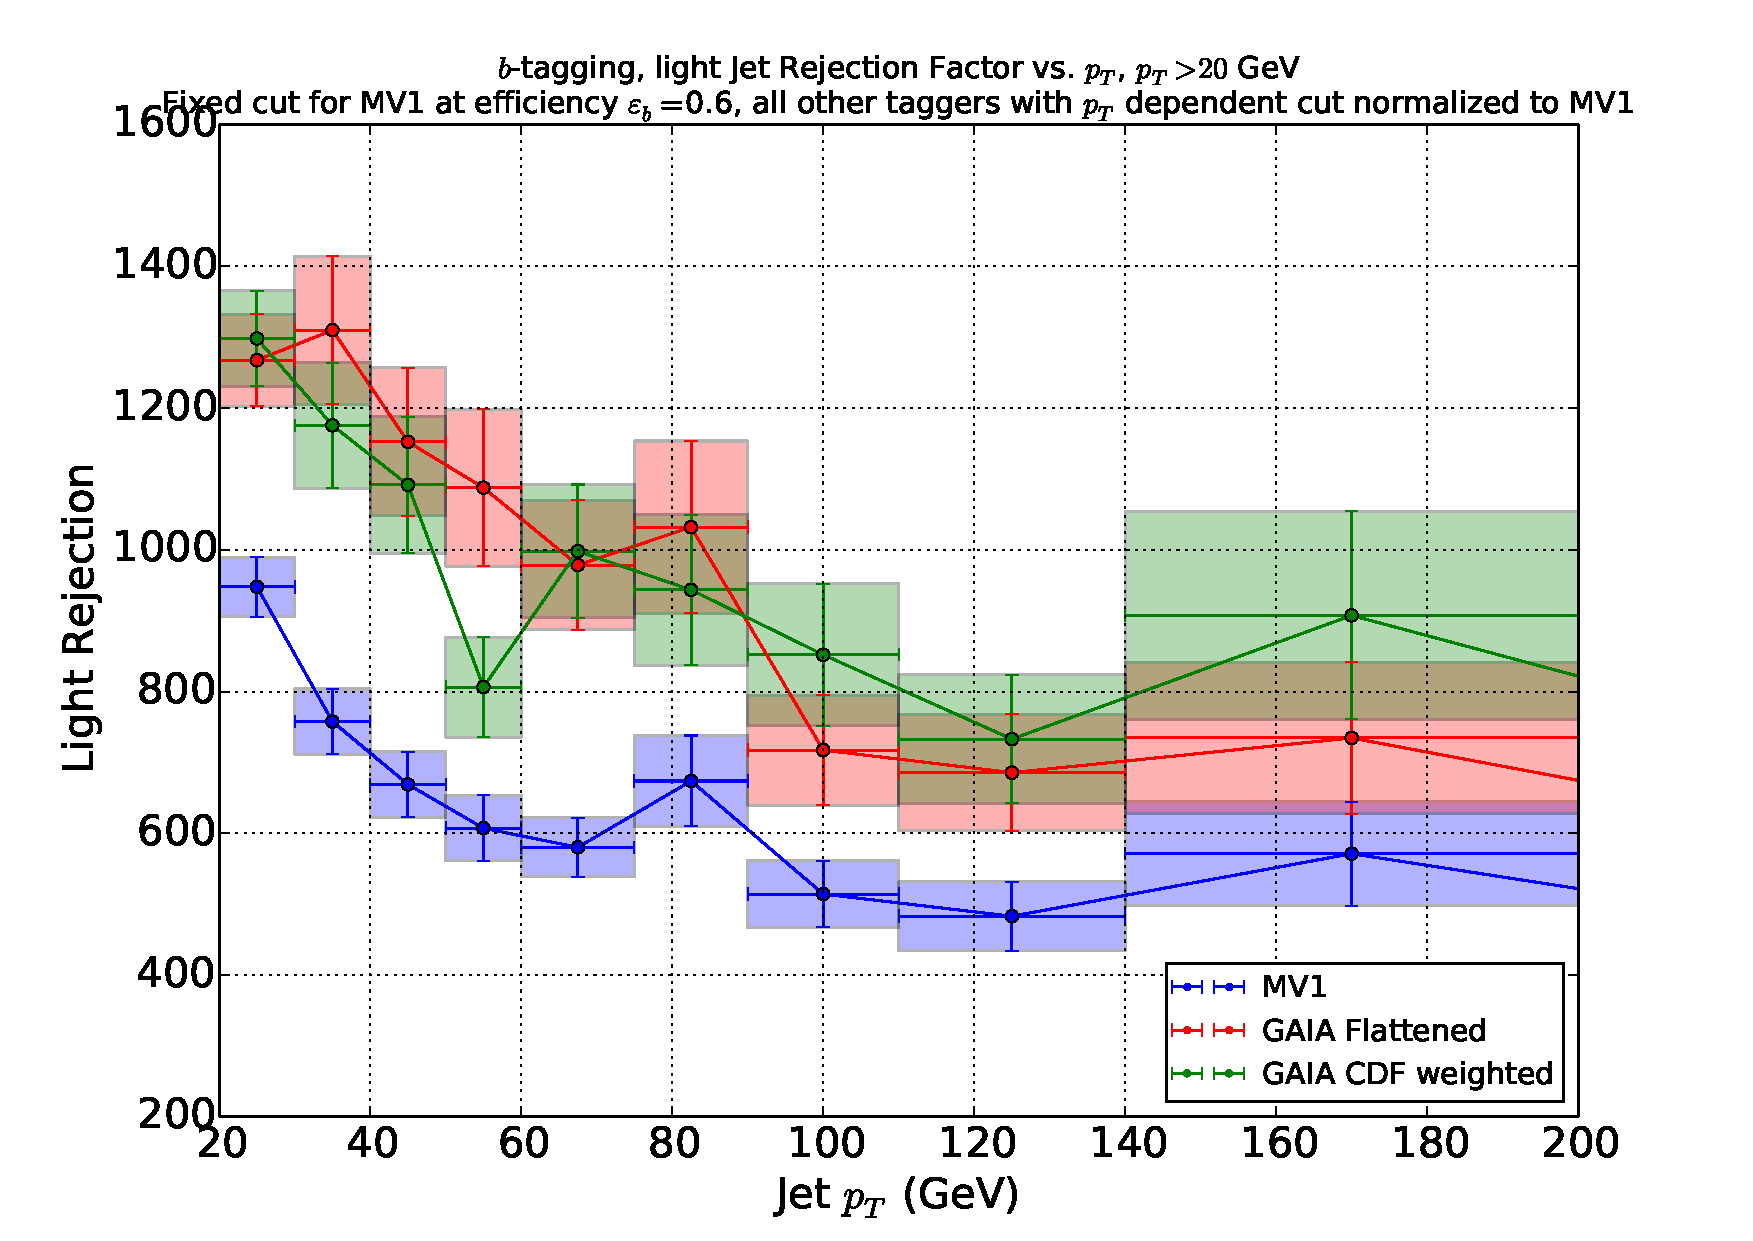
\includegraphics[width=\textwidth]{figures/btag/u_rej_mv1normalized_pTdep_60pct.pdf}
\caption[The ATLAS detector]{MV1 Normalized Performance of GAIA.
\label{fig:urejmv1norm60}}
\end{figure}

\begin{figure}
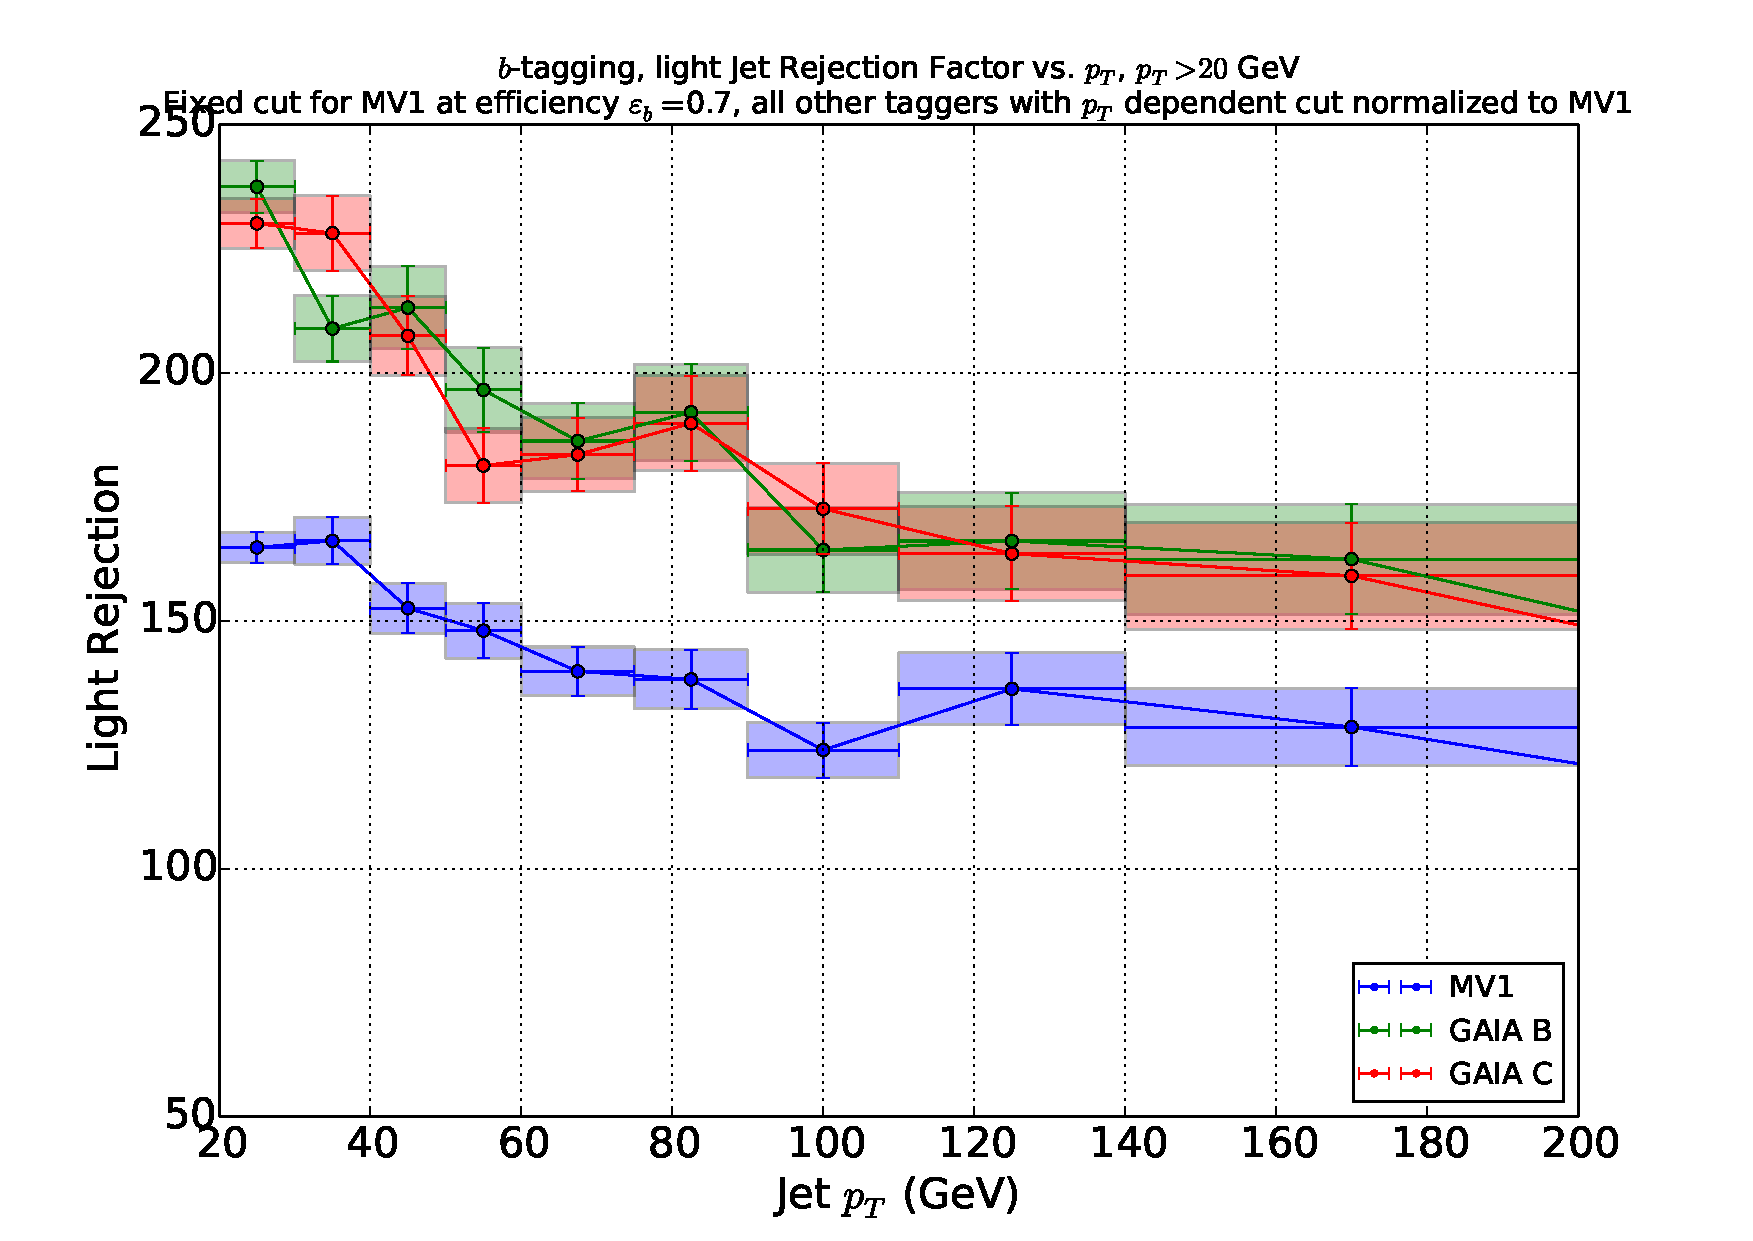
\includegraphics[width=\textwidth]{figures/btag/u_rej_mv1normalized_pTdep_70pct.pdf}
\caption[The ATLAS detector]{MV1 Normalized Performance of GAIA.
\label{fig:urejmv1norm70}}
\end{figure}



















%For each flavor $\theta$, we assume that
%\begin{equation}
%\label{eq:findingcut}
%\forall\omega\in [0,1], \exists \bar{p_\theta}\text{ such that }\int_0^{\bar{p_\theta}} f_\theta(x)dx = \omega.
%\end{equation}
%
%Since $f_\theta$ is a probability distribution, for each $\omega$ we want, the $\bar{p_\theta}$ is unique. Thus, we can define a function 







